%% 
%% Copyright 2019-2020 Elsevier Ltd
%% 
%% This file is part of the 'CAS Bundle'.
%% --------------------------------------
%% 
%% It may be distributed under the conditions of the LaTeX Project Public
%% License, either version 1.2 of this license or (at your option) any
%% later version.  The latest version of this license is in
%%    http://www.latex-project.org/lppl.txt
%% and version 1.2 or later is part of all distributions of LaTeX
%% version 1999/12/01 or later.
%% 
%% The list of all files belonging to the 'CAS Bundle' is
%% given in the file `manifest.txt'.
%% 
%% Template article for cas-sc documentclass for 
%% single column output.

%\documentclass[a4paper,fleqn,longmktitle]{cas-sc}
\documentclass[a4paper,fleqn]{cas-sc}

%\usepackage[numbers]{natbib}
%\usepackage[authoryear]{natbib}
\usepackage[authoryear,longnamesfirst]{natbib}
\usepackage[textsize=small]{todonotes}
%%%Author macros
\def\tsc#1{\csdef{#1}{\textsc{\lowercase{#1}}\xspace}}
\tsc{WGM}
\tsc{QE}
\tsc{EP}
\tsc{PMS}
\tsc{BEC}
\tsc{DE}
%%%

\begin{document}
	\let\WriteBookmarks\relax
	\def\floatpagepagefraction{1}
	\def\textpagefraction{.001}
	\shorttitle{Energy optimisation and adaptive coverage in WSN systems}
	\shortauthors{N Creech et~al.}
	%\begin{frontmatter}
	
	\title [mode = title]{Energy optimisation and adaptive coverage in WSN systems}                      
	
	\author[1]{Niall Creech\corref{cor1}}[type=editor,	orcid=0000-0002-9573-0991]
	\ead{niall.creech@kcl.ac.uk}
	\cortext[cor1]{Corresponding author}	
	\credit{Conceptualization of this study, Methodology, Software}
	
	\author[2]{Natalia Craido Pacheco\corref{cor2}}[]
	\ead{natalia.criado_pacheco@kcl.ac.uk}
	\credit{Supervision, Writing - Review and Editing}

	\author[3]{Simon Miles\corref{cor3}}[]
	\ead{simon.miles@kcl.ac.uk}
	\credit{Supervision, Writing - Review and Editing}

	\address[1]{Department of Informatics, King's College London, Bush House, Strand Campus, 30, Aldwych, London WC2B 4BG}
	\address[2]{Department of Informatics, King's College London, Bush House, Strand Campus, 30, Aldwych, London WC2B 4BG}
	\address[3]{Department of Informatics, King's College London, Bush House, Strand Campus, 30, Aldwych, London WC2B 4BG}
	


	\begin{abstract}
Lorem ipsum dolor sit amet, consectetur adipiscing elit, sed do eiusmod tempor incididunt ut labore et dolore magna aliqua. Ut enim ad minim veniam, quis nostrud exercitation ullamco laboris nisi ut aliquip ex ea commodo consequat. Duis aute irure dolor in reprehenderit in voluptate velit esse cillum dolore eu fugiat nulla pariatur. Excepteur sint occaecat cupidatat non proident, sunt in culpa qui officia deserunt mollit anim id est laborum.
\end{abstract}

%\begin{graphicalabstract}
%	
\includegraphics{figs/grabs.pdf}
%\end{graphicalabstract}
	
	\begin{highlights}
		\item Research highlights item 1
		\item Research highlights item 2
		\item Research highlights item 3
	\end{highlights}
	
	\begin{keywords}
		multi-agent system
		\sep multi-agent reinforcement learning
		\sep wireless sensor network
	\end{keywords}

	\newcommand{\acronymATARIA}[2]{ATA-RIA}
\newcommand{\acronymATARIAExtended}[2]{agent task allocation with risk-impact awareness (\acronymATARIA{}{})}
\newcommand{\acronymMGRAO}[2]{MG-RAO}
\newcommand{\acronymMGRAOExtended}[2]{multi-group resource allocation optimisation (\acronymMGRAO{}{})}
\newcommand{\acronymWSNOptimisation}[2]{AN-HTAO}
\newcommand{\acronymWSNOptimisationExtended}[2]{agent networks with hierarchical task allocation optimisation (\acronymWSNOptimisation{}{})}

\newcommand{\acronymWSNOptimisationSink}[2]{AN-HTAO (Sink agents)}
\newcommand{\acronymWSNOptimisationSinkExtended}[2]{agent networks with hierarchical task allocation optimisation, sink agents (\acronymWSNOptimisationSink{}{})}
\newcommand{\acronymWSNOptimisationArc}[2]{AN-HTAO (Task-path agents)}
\newcommand{\acronymWSNOptimisationArcExtended}[2]{agent networks with hierarchical task allocation optimisation, arc agents (\acronymWSNOptimisationArc{}{})}

\newcommand{\simulationSimple}[2]{\texttt{simple}}
\newcommand{\simulationExtended}[2]{\texttt{extended}}
\newcommand{\simulationNodeFailure}[2]{\texttt{node-failure}}


\newcommand{\algorithmSymbol}[2]{#1}
\newcommand{\algorithmBalanced}[2]{\algorithmSymbol{an-htao}{}}\newcommand{\algorithmBalancedSimple}[2]{\algorithmSymbol{an-htao}{} (simple)}
\newcommand{\algorithmBalancedExt}[2]{\algorithmSymbol{an-htao (extended)}{}}
\newcommand{\algorithmFailure}[2]{\algorithmSymbol{an-htao (failure)}{}}
\newcommand{\algorithmEnergy}[2]{\algorithmSymbol{an-htao (energy)}{}}
\newcommand{\algorithmQuality}[2]{\algorithmSymbol{an-htao (quality)}{}}
\newcommand{\algorithmDistribution}[2]{\algorithmSymbol{an-htao (distribution)}{}}
\newcommand{\algorithmQRouting}[2]{\algorithmSymbol{q-routing}{}}
\newcommand{\algorithmQRoutingSimple}[2]{\algorithmSymbol{q-routing}{}(simple)}
\newcommand{\algorithmQRoutingExt}[2]{\algorithmSymbol{q-routing}{} (extended)}
\newcommand{\algorithmQRoutingFailure}[2]{\algorithmSymbol{q-routing}{} (failure)}

\newcommand{\algorithmBaseline}{\algorithmQRouting{}{}}
\newcommand{\acronymQRouting}[2]{Q-Routing}


	\section{Introduction}

\todo[inline]]{Why is the subject/problem area important?}
\textit{Wireless sensor networks (WSNs)} have many applications and research studies in areas such as environmental monitoring, agriculture, and military uses (See Table \ref{table:applications}). More recently, the availability and lower cost of low-power wireless transmitters \citep{902661}, solar-harvesting components \citep{Prauzek2018}, and micro-electro-mechanical systems \citep{1045391} has allowed large deployments sizes and scope of use, expanding their real-world use and opening up new areas for practical research \citep{Kandris2020}.

\begin{table}[h]
	\footnotesize
\begin{tabular}{|p{0.2\textwidth}|p{0.2\textwidth}|p{0.5\textwidth}|}
\hline
Area & References & Summary \\
\hline
Ocean monitoring and the marine environment & \cite{Mahdy2008a, Albaladejo2010, 6973877} & XXX \\
Radiation contamination & \cite{Gomez2015} & XXX \\
 Water quality & \cite{Fang2010} & XXX \\
Agriculture  & \cite{8745854} & XXX \\
Volcano monitoring  & \cite{Werner-Allen2006} & XXX \\
Flood monitoring  & \cite{Castillo-effen2004} & XXX \\
Military & \cite{6268958} & XXX \\
\hline
\end{tabular}
\caption{Real-world applications of wireless sensor networks}
\label{table:applications}	
\end{table}

\todo[inline]{Why are these important? Uses?}

\todo[inline]{What are the current solutions, what are the problems and how are we improving them?}

\todo[inline]{What is the solution and contributions we present?}
Based on the algorithms presented by the authors \citep{creech2021dynamic, creech2021resource}.
\todo[inline]{Summarise the structure of the paper}




	\newtheorem{thm}{Theorem}
	\newdefinition{definition}{Definition}

	\maketitle
	
	\section{Introduction}

\todo[inline]]{Why is the subject/problem area important?}
\textit{Wireless sensor networks (WSNs)} have many applications and research studies in areas such as environmental monitoring, agriculture, and military uses (See Table \ref{table:applications}). More recently, the availability and lower cost of low-power wireless transmitters \citep{902661}, solar-harvesting components \citep{Prauzek2018}, and micro-electro-mechanical systems \citep{1045391} has allowed large deployments sizes and scope of use, expanding their real-world use and opening up new areas for practical research \citep{Kandris2020}.

\begin{table}[h]
	\footnotesize
\begin{tabular}{|p{0.2\textwidth}|p{0.2\textwidth}|p{0.5\textwidth}|}
\hline
Area & References & Summary \\
\hline
Ocean monitoring and the marine environment & \cite{Mahdy2008a, Albaladejo2010, 6973877} & XXX \\
Radiation contamination & \cite{Gomez2015} & XXX \\
 Water quality & \cite{Fang2010} & XXX \\
Agriculture  & \cite{8745854} & XXX \\
Volcano monitoring  & \cite{Werner-Allen2006} & XXX \\
Flood monitoring  & \cite{Castillo-effen2004} & XXX \\
Military & \cite{6268958} & XXX \\
\hline
\end{tabular}
\caption{Real-world applications of wireless sensor networks}
\label{table:applications}	
\end{table}

\todo[inline]{Why are these important? Uses?}

\todo[inline]{What are the current solutions, what are the problems and how are we improving them?}

\todo[inline]{What is the solution and contributions we present?}
Based on the algorithms presented by the authors \citep{creech2021dynamic, creech2021resource}.
\todo[inline]{Summarise the structure of the paper}




	\section{Related work}
\label{section:background}

\textit{Wireless sensor networks (WSNs)} are collections of independent, battery-powered nodes connected through wireless transmission, often used to monitor a geographical area using sensors \citep{Akyildiz,Yick2008a}. In many circumstances the areas under study are difficult to access, such as remote locations, ocean-based studies, or contaminated areas. \textit{Environmental wireless sensor networks (E-WSNs)} in particular are characterised by intermittent connectivity between nodes, and harsh environmental conditions that lead to degradation of the network, so that it must adapt in response to these changes to maintain its functionality \citep{Oliveira2011}. The energy sources for nodes are commonly non-replaceable batteries, and the nodes' dispersal ad-hoc, making a high level of autonomous communication, coordination, and power consumption management, essential. WSNs can consist of static sensor deployments, or as mobile agents, adding to the need for adaptation in the network \citep{ramasamy2017mobile, 4224091}. Sensors are usually small and inexpensive, capable of utilising limited compute and storage resources. They have one or multiple sensing devices to take measurements from the environment, ranging through chemical, optical, thermal, biological, and radioactivity detection. This collected data can then be transmitted to a base station and retransmitted to be stored remotely and analysed.

\subsection{Requirements for a WSN}
In realistic scenarios, there are five key requirements that each present challenges in deploying and operating a WSN system.
\begin{enumerate}
\item \label{requirement:energy}\textit{Energy consumption.} Each node in a WSN network has limited power available to function supplied by a battery. Depending on the environmental conditions, there may be some form of energy-capture component built into each node, such as solar-harvesting \citep{Prauzek2018}. However, even with this additional energy replenishment, energy is limited, and will eventually be exhausted. Batteries cannot be manually replaced in remote or inhospitable locations, that are often the focus of WSN deployments, so minimising energy consumption is essential \citep{Anastasi2009}. This can be done through the use of low-power components, \citep{4772585, 8108667}, as well as applying energy-aware routing protocols amongst nodes \citep{s90100445}. 

\item \label{requirement:quality} \textit{Quality of measurement data.} A node taking a reading may have a faulty sensor, leading to variations in the recorded values and lack of reliability. Sensors may get more accurate readings using more energy or longer time scales, for example, as the sampling time of a temperature or radiation sensor is increased, the more accurate the reading \citep{s17061221}. Therefore nodes must trade-off the quality of its data acquisition with the restricted amount of energy available to it across its lifetime \citep{7845391}.

\item \label{requirement:coverage} \textit{Coverage of sensors.} In many environmental situations sensors are distributed in an ad-hoc manner, meaning their distribution is initially unknown amongst the nodes. Sensors may also have occlusion problems due to the topography of the environment or objects blocking connectivity or measurement \citep{10.1007/978-3-540-69170-9_23}. Therefore, to initialise the system, the deployed nodes must find which other nodes to communicate with that will allow all the locations targeted by readings to be covered. They must also be resilient to temporary or permanent outages on the network that require re-routing connectivity to maintain this coverage.

\item \label{requirement:resilience} \textit{Network resilience.} Wireless sensor networks add substantial additional risks to reliability over standard networking. Nodes are at risk of running out of power or of component failure, often exacerbated by harsh conditions. Environmental effects or obstacles may physical impact transmission or reception of signals. Loss of communication to a node is especially impactful as there are often multi-hop routes involved, which multiplies the risks \citep{Paradis2007}. To mitigate this problem, the WSN must be able to reconfigure its routing pathways to work around nodes are no longer functioning so that the needed sensor nodes can still be reached.

\item \label{requirement:lifetime} \textit{System lifetime.} Whether due to the impact of environmental degradation, power exhaustion, or connectivity loss, nodes in a network have a limited useful lifespan \citep{Mak2009}. As nodes are lost, the system itself becomes degraded. Eventually it is unable to achieve its goals to a sufficient quality to be useful, defining the systems' lifetime. To extend this lifetime as far as possible we try to reduce the wear on nodes, principally, by ensuring that energy consumption is distributed through out the system evenly \citep{BABAYO20171176, Engmann2018}.
\end{enumerate}
To summarise, we require that WSNs minimise their energy usage, distribute component usage to increase their working lifetime, provide measurements of sufficient quality that cover the required area, and adapt to network disruptions to maintain these properties.

\subsection{Algorithmic approaches}
The best network connectivity, task allocation strategy, and assignment of resource by agents are unknown at system initialisation. These values may also vary throughout the systems' lifetime. Due to this, there has been increasing research into algorithms utilising reinforcement learning techniques that can learn these values as the system evolves \citep{Al-Rawi2015}. These broadly contain two main challenges. First, how algorithms can best learn to optimise across multiple system goals. Second, how agents' share information and cooperate to connect their localised actions to the broader system goals. In the first case, an approach has been to enhance network routing protocols with Q-learning, using a reward function that consider multiple factors including residual energy, link distance, and hop count, to select better routes while increasing the lifetime of the network and energy efficiency \citep{Guo2019}. 

\paragraph{Evolutionary algorithms}
\reviewquestionopen{You imply (paragraph 3) that two research groups, Li and Zhang 2009 and Sengupta et al. 2013, have provided solutions to multi-objective optimisation in WSNs. It's not clear how the goal of this paper as expressed in the final paragraph differs from that. If so, what don't they solve that you will?
}

\reviewtodo{
Multi-Objective Differential Evolution with Adaptive Control of Parameters and Operators \citep{Ke2011}\\
A Brief Review on Multi-objective Differential Evolution \citep{Mohd2020}\\
Differential Evolution: A survey of theoretical analyses \citep{Opara2019}\\
Differential Evolution Algorithm: Recent Advances \citep{Suganthan2012}\\
Differential Evolution in Agent-Based Computing \citep{Godzik2019}.\\
Self-adaptive Differential Evolution \citep{Omran2005}\\
An Evolutionary Multiagent Framework for Multiobjective Optimization \citep{Zhang2020a}.\\
Differential Evolution algorithm applied to non-stationary bandit problem \citep{StPierre2014}\\
Self-adaptive, multi-population differential evolution in dynamic environments \citep{Novoa-Hernandez2013}\\
Autonomous and fault tolerant vehicular self deployment mechan     isms in MANETs \citep{Gundry2013}\\
Research status of multi - robot systems task allocation and uncertainty treatment \citep{Li2017}\\
{Multi-agent System Based on Self-adaptive Differential Evolution for Solving Dynamic Optimization Problems} \citep{Cep2017}\\
Differential Evolution for Lifetime Maximization of Heterogeneous Wireless Sensor Networks \cite{Xu2013}
}


This problem of optimising WSN systems across multiple objectives is further detailed in work by \cite{ s150717572}, with the multi-objective evolutionary algorithm techniques developed going on to be integrated into algorithms for the WSN domain \citep{4633340,SENGUPTA2013405}. In particular, \textit{differential evolution (DE)} \cite{XXX} techniques have proven a simple and effective way of optimising multi-agent systems \cite{XXX}, and have been utilised in both multi-objective \cite{XXX}, and non-stationary \cite{XXX} systems. However, there are a number of factors that can make DE less applicable in real-world situations;
\begin{itemize}
	\item \textit{Occlusion and obstruction} Nodes in a WSN may be obstructed by other objects or weather effects in an environment, making some actions less optimal or even possible. e.g, a transmission action blocked by a rock.

	\item \textit{Communication bandwidth limitations} WSN nodes usually have limited transmission bandwidth and processing power, so exchanging significant amounts of information to apply algorithms is not possible. 
	
	\item \textit{Reliability of centralised coordination} Using a centralised node to compute evolutions will involve significant data transfer, with nodes required to relay data in larger systems due to transmission strength. In addition, connectivity to such a node may be intermittent. 
	
	\item \textit{Heterogeneity of nodes} Nodes may be homogenous in specification at system initialisation, however, localised conditions, ad-hoc placement, and changing functionality over time, differentiates their capabilities and optimal actions over time. e.g, the degradation in transmission power as a nodes battery wears.
	
	\item \textit{Uniqueness due to location} Each nodes' optimal actions are often unique, for example, localised sensing conditions. e.g. a node in an ocean-based WSN may have its temperature sensor placed in a strong current, with rapidly variable readings.
	
	\item \textit{Mobility} Nodes may be mobile to different degrees, with this changing throughout the systems lifetime. A nodes optimal policy one moment may change as its mobility changes, and two identical nodes may have widely different optimal actions to take based on their speed and direction of movement. e.g \todo[inline]{Put an example here}  
\end{itemize}
For these reasons, we focus on distributed reinforcement learning techniques.

\paragraph{Distributed reinforcement learning}
For the second problem, there has been work looking at cooperative Q-learning between nodes for better task scheduling and energy consumption \citep{doi:10.1155/2014/765182}. Due to the increased resources and computation required to coordinate amongst multiple agents and form cooperative behaviours, we look more to approaches using decentralised, autonomous agents learning from localised knowledge only \citep{10.1007/978-3-642-11814-2_4}.  This utilises the idea of individual agents optimising energy usage within a small neighbourhood of nearby nodes to optimise the energy consumption of the system as a whole. 

Each of these solutions mentioned above cover elements of the desired behaviours of a WSN. We take these key concepts from that work and build upon them.
\reviewquestion{Second list, item 2: It is odd that it ends with a citation to Mihaylov et al. when you are talking about what the focus of your own is (and you aren't called Mihaylov). It is not clear what the citation is providing the source for.
}
\reviewquestion{Second list, item 3: The last sentence is overly complex and seems to be describing optimisation for two competing things (quality of task completion and utility of the system overall). I suggest it should be reduced to something like "The algorithm should be able to learn the allocation of resources at each node that optimises overall system utility."
}
\begin{enumerate}
	\item \textit{The optimisation of multiple objectives}.  The algorithm must be able to balance learning to take actions that benefit more than one objective so that it can optimise across energy use, task quality, etc and meet the needs of a WSN \citep{Guo2019, s150717572, SENGUPTA2013405}.

	\item \textit{The decentralisation of coordination}. With limited resources for transmission and computation, nodes in WSN networks must minimise the explicit coordination of agents.  In harsh environments, and the removal of manual maintenance, centralised coordination or knowledge becomes both difficult and a risk to system robustness \cite{XXX}.
	
	\item \textit{The localisation of agent knowledge}. Nodes have limits on transmission range and bandwidth, causing them to be restricted to information available nearby \citep{10.1007/978-3-642-11814-2_4}. For this reason, we focus on using only the knowledge in an agents' local neighbourhood in our algorithm, and use this to generate optimisation in the system as a whole.
	
	\item \textit{The allocation of node resources}. As described, nodes in a WSN have limited resources with which to complete their tasks. Each nodes' preference of how its available resources are allocated amongst the tasks allocated to it will have an effect on task completion quality. The algorithm should be able to learn the allocation of resources at each node that optimises overall system utility. 
\end{enumerate}

\subsection{Summary}
We look to improve on previous work by developing an algorithm that is able to cover all of the key requirements described above effectively, while still giving flexibility in the optimisation balance between each of them. By setting the system objectives as the minimisation of energy consumption, and the maximisation of system lifetime, measurement quality, and sensor coverage, we can define the problem as a multi-objective learning problem in a distributed multi-agent system. In the next section we formalise the terminology, definitions, and the problem we look to address.



	\section{Balancing energy and measurement in a WSN system}
\label{section:problem}
%%%%%%%%%%%%%%%%%% NOTATION %%%%%%%%%%%%%%%%%%%%%%%%%%
\newcommand{\varTime}[2]{\phi}
\newcommand{\setTime}[2]{\Phi}
\newcommand{\varAtomicTask}[2]{\varSymbol{at}{#1}{#2}}
\newcommand{\setAtomicTask}[2]{\setSymbol{AT}{#1}{#2}}
\newcommand{\varCompositeTask}[2]{\varSymbol{ct}{#1}{#2}}
\newcommand{\setCompositeTask}[2]{\setSymbol{CT}{#1}{#2}}

\newcommand{\varAgent}[2]{g_{#1}^{#2}}
\newcommand{\setAgents}[2]{G_{#1}^{#2}}

\newcommand{\powerSetAgents}[2]{\powerSetSymbol{G_{#1}^{#2}}{}{}}
\newcommand{\varIdleAgent}[2]{\varAgent{i}{}}  
\newcommand{\varSleepAgent}[2]{\varAgent{s}{}}  
\newcommand{\varChildAgent}[2]{\varAgent{c}{}}    
\newcommand{\varParentAgent}[2]{\varAgent{p}{}}

\newcommand{\varOrchestrationEnergy}[2]{e_{orch}}
\newcommand{\varTransmissionEnergy}[2]{e_{trans}}
\newcommand{\varReceiverEnergy}[2]{e_{recv}}
\newcommand{\varSensorEnergy}[2]{e_{sens}}
\newcommand{\varIdleEnergy}[2]{e_{idle}}
\newcommand{\functionTaskRange}[2]{
	\functionSignature{\mathit{range}}
	{\varAtomicTask{}{}}
}


\newcommand{\functionAtomicTaskEnergyConsumptionSignature}[2]{
	\functionSignature{atec}{\varAtomicTask{}{}}}

\newcommand{\formalAtomicTaskEnergyConsumption}[2]{
	\functionFormal{atec}
	{\setAtomicTask{}{}}
	{\setRealNumbersNonNegative{}{}}}
%%%%%%%%%%%%%%%%%%%%%%%
\newcommand{\symbolDataAcquisition}[2]{\setSymbol{DAQ}{#1}{#2}}
\newcommand{\symbolTransmission}[2]{\setSymbol{TX}{#1}{#2}}
\newcommand{\symbolReceiver}[2]{\setSymbol{RX}{#1}{#2}}
\newcommand{\symbolWakeUpRadio}[2]{\setSymbol{WUR}{#1}{#2}}


\newcommand{\functionSystemEnergyDistribution}[2]{
	\functionSignature{sed_{\varTime{}{}}}
	{\setAgent{}{}}
}
\newcommand{\functionSystemEnergyVariability}[2]{
	\functionSignature{sev_{\varTime{}{}}}
	{\setAgents{}{}}
}
\newcommand{\functionAgentEnergyTotal}[2]{
	\functionSignature{aet_{\varTime{}{}}}
	{\varAgent{#1}{#2}}
}

\newcommand{\functionProbabilityInit}[2]{
	\functionSignature{pinit}{\varAgent{}{}}
}
\newcommand{\functionProbabilityRand}[2]{
	\functionSignature{prand}{\varAgent{}{}}
}
\newcommand{\functionProbabilityWear}[2]{
	\functionSignature{pwear}{\varAgent{}{}}
}
\newcommand{\functionProbabilityFail}[2]{
	\functionSignature{pfail}{\varAgent{}{}}
}
\newcommand{\varConstantInit}[2]{{C}{INIT}^{#2}}
\newcommand{\varConstantRand}[2]{{C}{RAND}^{#2}}
\newcommand{\varConstantWear}[2]{{C}{WEAR}^{#2}}
\newcommand{\varEnergyInit}[2]{{E}{INIT}^{#2}}
\newcommand{\varEnergyWear}[2]{{E}{WEAR}^{#2}}

%%%%%%%%%%%%%%%%%% NOTATION %%%%%%%%%%%%%%%%%%%%%%%%%%
\newcommand{\varSample}[2]{\varSymbol{\psi}{#1}{#2}}
\newcommand{\setSample}[2]{\setSymbol{\Psi}{#1}{#2}}
\newcommand{\varMeasurement}[2]{\varSymbol{m}{#1}{#2}}
\newcommand{\varPeriod}[2]{\varSymbol{p}{#1}{#2}}
\newcommand{\varError}[2]{\varSymbol{\omega}{#1}{#2}}
\newcommand{\setError}[2]{\setSymbol{\Omega}{#1}{#2}}
\newcommand{\tupleVarSample}[2]{
	(\varTime{#1}{#2}, \varMeasurement{#1}{#2}, \varError{#1}{#2})
}
\newcommand{\tupleSetSample}[2]{
	(\setTime{#1}{#2}, \setMeasurement{#1}{#2}, \setError{#1}{#2})
}

%%%%%%%%%%%%%%%%%% NOTATION %%%%%%%%%%%%%%%%%%%%%%%%%%
\newcommand{\varBatteryEnergy}[2]{\varSymbol{e}{\varAgent{}{}}{#2}}
\newcommand{\setBatteryEnergy}[2]{\setSymbol{E}{#1}{#2}}
\newcommand{\varBatteryEnergyMax}[2]{\varBatteryEnergy{\varAgent{}{}}{max}}

%%%%%%%%%%%%%%%%%%%%%%%%%%%%%%%%%%%%%%
\newcommand{\varLocation}[2]{\varSymbol{loc}{#1}{#2}}
\newcommand{\setLocation}[2]{\setSymbol{LOC}{#1}{#2}}
\newcommand{\formalVarLocation}[2]{(x,y)}
\newcommand{\formalSetLocation}[2]{(\setRealNumbers{}{} \times \setRealNumbers{}{})}

\newcommand{\functionDeployment}[2]{
	\ifx \\1\\
	\functionSignature{conf}{\setAgents{}{}}
	\else
	\functionSignature{conf}{#1}
	\fi 
}
\newcommand{\formalDeployment}[2]{\functionFormal{conf}{\setAgents{}{}}{(\setRealNumbersNonNegative{}{} \times \setRealNumbersNonNegative{}{})}}
\newcommand{\functionTaskArc}[2]{\functionSignature{path}{\varAtomicTask{}{}}}
\newcommand{\formalTaskArc}[2]{\functionFormal{path}{\setAtomicTask{}{}}{\powerSetAgents{}{}}}
\newcommand{\functionTaskDemandPoint}[2]{\functionSignature{dp}{\varAtomicTask{}{}}}
\newcommand{\formalTaskDemandPoint}[2]{\functionFormal{dp}{\setAtomicTask{}{}}{(\setRealNumbersNonNegative{}{} \times \setRealNumbersNonNegative{}{})}}
\newcommand{\varActiveAgent}[2]{\varAgent{#1}{\oplus}}
\newcommand{\varInactiveAgent}[2]{\varAgent{#1}{\ominus}}
\newcommand{\varSensingAgent}[2]{\varAgent{#1}{\ast}}
\newcommand{\varSinkAgent}[2]{\varAgent{#1}{\Delta}}

\newcommand{\varEnergy}[2]{\varSymbol{e}{#1}{#2}}
\newcommand{\setEnergy}[2]{\setSymbol{E}{#1}{#2}}
%%%%%%%%%%%%%%%%%%%%%%%%%%%%%%%%%%%%%
\newcommand{\varResource}[2]{\varSymbol{r}{#1}{#2}}
\newcommand{\setResource}[2]{\setSymbol{R}{#1}{#2}}
\newcommand{\formalTaskResourceAllocation}[2]{
	\functionFormal{ra}
	{\setAgents{}{} \times \setAtomicTask{}{}}
	{\powerSetSymbol{\setResource{}{} \times \setRealNumbersNonNegative{}{}}{}{}}
}
\newcommand{\functionTaskResourceAllocation}[2]{
	\functionSignature{ra}
	{\varAgent{}{}, \varAtomicTask{}{}}
}
%%%%%%%%%%%%%%%%%%%%%%%%%%%%%%%%%%%%%%%%
	\section{Solving the multi-objective WSN problem}
\label{section:solution}
As defined in the previous section, we are looking for a method to optimise multiple objectives in our WSN system. To do so we will incorporate two algorithms, the \acronymATARIAExtended{}{} and \acronymMGRAOExtended{}{} algorithms. We give the high-level purpose and requirements of each algorithm in the next sections, however, full details and theoretical justification can be found in \cite{creech2021dynamic, creech2021resource}.

\subsection{Optimisation algorithms for task allocation and resource allocation}
\label{section:algorithm_summaries}
%%%%%%%%%%%%%%%%
\newcommand{\varAction}[2]{\varSymbol{a}{#1}{#2}}
\newcommand{\functionExec}[2]{\texttt{exec}(\varAtomicTask{}{})}
\newcommand{\functionAlloc}[2]{\texttt{alloc}(\varAtomicTask{}{}, \varAgent{}{})}
\newcommand{\functionInfo}[2]{\texttt{info}(\varAgent{}{})}
\newcommand{\functionLink}[2]{\texttt{link}(\varAgent{}{})}
\newcommand{\functionATARIA}[2]{
	\functionSignature{
		ataria_{\varAgent{}{}}
	}{
		\varAtomicTask{}{}, \varAgent{self}{}
	}
}	
\newcommand{\formalATARIA}[2]{
	\functionFormal{\texttt{ataria}_{\varAgent{}{}}}
	{\setAtomicTask{}{} \times \setAgents{}{}}
	{
	\texttt{exec}(\setAtomicTask{}{})
	\times \texttt{alloc}(\setAtomicTask{}{}, \setAgents{}{})
	\times \texttt{info}(\setAgents{}{})
	\times \texttt{link}(\setAgents{}{})
}
}
\newcommand{\functionMGRAOWeighting}[2]{\texttt{mgrao-weight}(\varAtomicTask{}{}, \varAgent{self}{})}
\newcommand{\formalMGRAOWeighting}[2]{
	\functionFormal{\texttt{mgrao-weight}_{\varAgent{}{}}}
	{\setAtomicTask{}{} \times \setRealNumbers{}{}}
	{
		\setRealNumbers{}{}
	}
}
\newcommand{\functionMGRAOUpdate}[2]{
	\texttt{mgrao-update}_{\varAgent{}{}}
	(\varAtomicTask{}{}, \functionTaskAbsoluteValue{}{})}
\newcommand{\formalMGRAOUpdate}[2]{
	\functionFormal{\texttt{mgrao-update}_{\varAgent{}{}}}
	{\setAtomicTask{}{} \times \setRealNumbers{}{}}
	{
		\setRealNumbers{}{}
	}
}
%%%%%%%%%%%%
	
The \acronymATARIA{}{} algorithm enables agents in the system to learn the best actions to take given their current state. This ranges from deciding which other agents to allocate tasks to and obtain the best composite task values, to exploring the system for other agents, while adapting connectivity to handle network disruption. An agent uses the \acronymATARIA{}{} algorithm to choose an action to take, which can be one of the following,
\begin{enumerate}
	\item $\functionExec{}{}$, The agent will execute the atomic task $\varAtomicTask{}{}$ itself.
	\item $\functionAlloc{}{}$, the agent will allocate the atomic task $\varAtomicTask{}{}$ to another agent $\varAgent{}{}$.
	\item $\functionInfo{}{}$, the agent will request information from another agent $\varAgent{}{}$.
	\item $\functionLink{}{}$, the agent will allocate resources to hold information on the agent $\varAgent{}{}$ and maintain a connection.
\end{enumerate}
The \acronymATARIA{}{} algorithm learns to select the actions that generate the best composite task values, and adapt the choice of action depending on how good the composite task values are in comparison to the historical values through the updating of Q-values in its temporal-update algorithm. The algorithm will select one of the possible actions for the agent $\varAgent{}{}$, given it has non-completed, allocated tasks $\setAtomicTask{}{}$, and knows of other agents $\setAgents{}{}$ through the function,
\begin{equation}
\label{eq:ataria}\formalATARIA{}{}
\end{equation}

To enable agents to form arcs we allow atomic tasks that have been allocated to an agent to be either executed by that agent, or re-allocated to further agents, through running the \acronymATARIA{}{} algorithm. Figure \ref{fig:arc-flow} illustrates an arc where there are two re-allocations made before a specific atomic task is allocated to an agent that completes the task by taking a measurement.
\begin{figure}[ht]
	\centering
	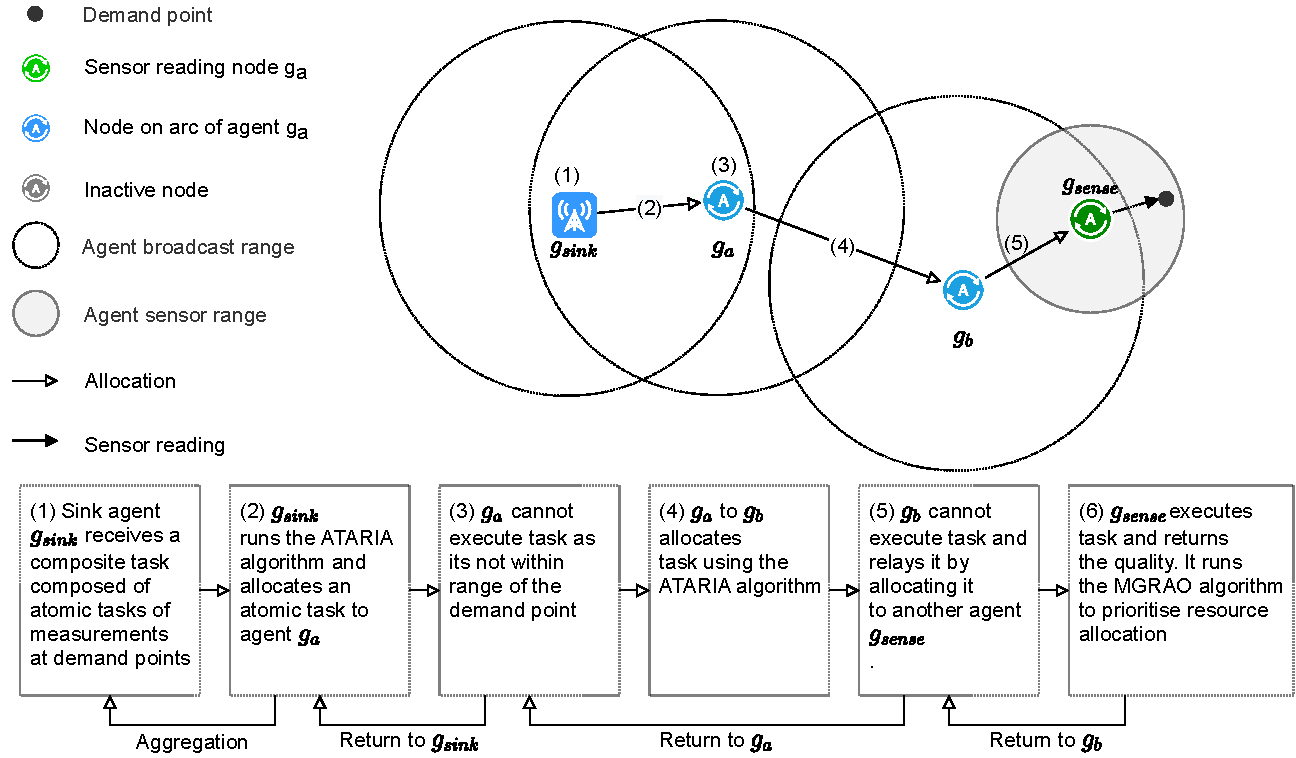
\includegraphics[width=0.8\linewidth, trim={25pt 0pt 25pt 0pt, clip}]{arc-flow}
	\caption{\textbf{Allocation along an arc}. This diagram illustrates how allocations can be relayed along an arc using successive applications of the \acronymATARIA{}{} algorithm.}
	\label{fig:arc-flow}
\end{figure}

The \acronymMGRAO{}{} algorithm helps agents executing atomic tasks allocate their resources to optimise the corresponding composite task value. This has two parts, an update algorithm that adjusts weights of resources based on received atomic task values, $\label{eq:mgrao_update}\formalMGRAOUpdate{}{}$,  and the application of these weights to generate the task execution quality itself, $\label{eq:mgrao_weighting}\formalMGRAOWeighting{}{}$. The update algorithm will change the resource weightings for an agent, $\functionAgentResources{}{}$, given the type of an atomic task completed, and the its absolute task value to the corresponding composite task. The weighting algorithm simply returns the resource weighting for calculation of an atomic tasks' quality $\functionAtomicTaskQualitySignature{}{}$ on its completion.


	\subsection{Configuration}

We simulated two systems to evaluate the algorithms in four different configurations (See Figure \ref{fig:system-types}).

\begin{figure}[ht]
	\centering
	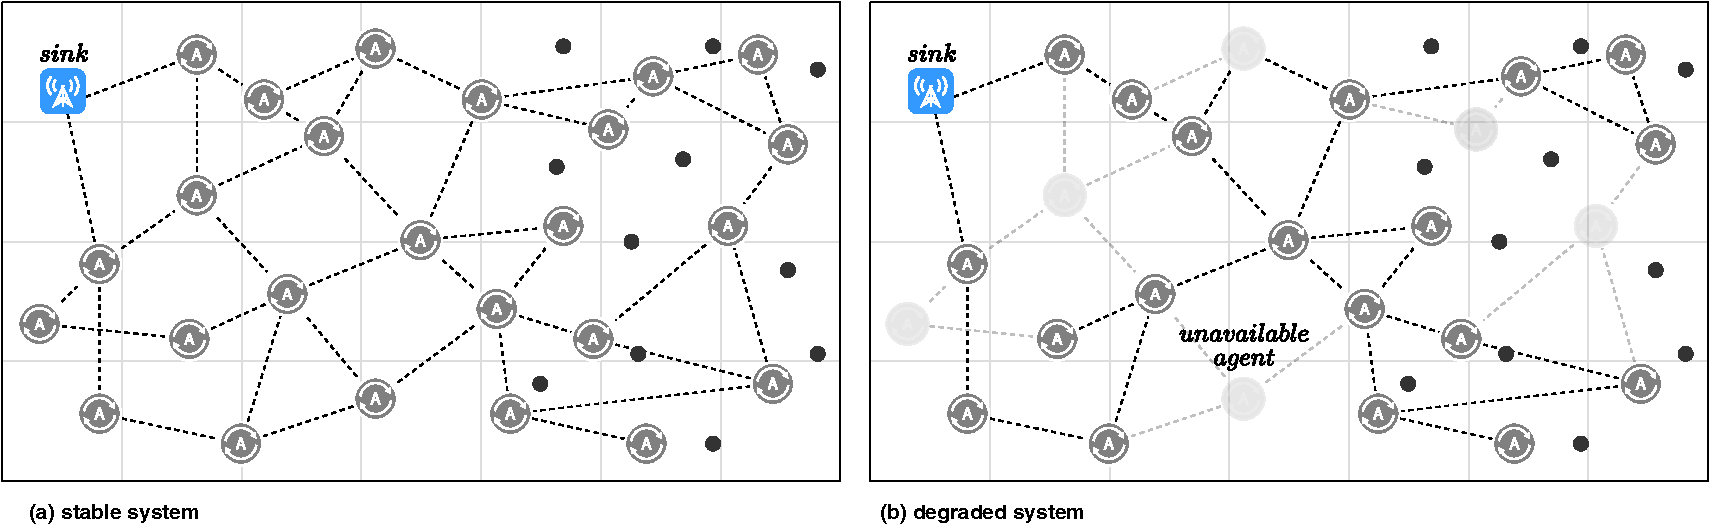
\includegraphics[width=0.9\linewidth]{system-types}
	\caption{\textbf{System types}. The diagram shows examples of the two systems. In the first \simulationSimple{}{}, there are $10$ possible agents that can execute the measurement task, tasks' demand points are distributed across the map. In the second, \simulationExtended{}{} system, there are $25$ agents that can execute the measurement tasks. The tasks' demand points are clustered away from the sink node.}
	\label{fig:system-types}
\end{figure}

The \simulationSimple{}{} system  equal weighting for each of the CTV components $\alpha, \beta, \gamma$ (Eq. \ref{eq:ctv}). The sink node was given $5$ measurement tasks to complete from outside the system, repeated $3$ times before one episode was complete. $10$ nodes were distributed randomly in the system, each capable of completing a task, or allocating it to any of $3$ nodes it was connected to. Each node could complete any measurement task with a quality dependent on their closeness to the demand point associated with the task (Eq. \ref{eq:atomic_task_quality}). The energy of all nodes in the system was fully reset at the end of each episode. An example of the simple system layout can be seen in Figure \ref{fig:system-types}(a). 

The \simulationExtended{}{} system had CTV component weightings where each of the relevant properties were given an $80\%$ dominance over the value of CTV value. The sink node was given $10$ measurements to allocate, with no repetition. It was also placed at a significantly large distance from the demand points associated with the tasks. $25$ nodes were distributed randomly in the system. This system examined the impact of the algorithm optimising the allocation of tasks towards the goals stated in Section \ref{section:optimisation_problem}. Task value could be maximised, but at the cost of longer arcs and therefore energy usage, or lower task values, and lower energy consumption. Figure \ref{fig:route_types} illustrates these two route types for task completion.

\subsection{Results}
Labels and descriptions for the algorithms are shown in Table \ref{table:summary_of_algorithms}, with configuration in Table \ref{table:summary_of_configurations}. Results for the \algorithmBalanced{}{} algorithm in the \simulationSimple{}{} system, and the \algorithmEnergy{}{}, \algorithmQuality{}{}, \algorithmDistribution{}{} algorithms in the \simulationExtended{}{} system are shown in Table \ref{table:results}.

System utility percentages show the summed values of composite tasks per episode (Eq. \label{eq:system_utility}) as compared to the theoretical maximum utility in the system \footnote{Note that the theoretical maximum is not necessarily attainable in all systems, dependent on their randomised node configurations.}. Energy available is presented as a percentage of that of a system containing nodes with full battery charge. We compare the different biases for optimisation across the CTV components of task values, energy availability, and distribution using quality-energy percentages. These use the available energy component in as a baseline, and show the percentage increase or decrease in average task qualities. Task-distribution shows the variation in the agents completing tasks, i.e. $\funcSize{set(\setAgents{}{})}{}/\funcSize{\setAgents{}{}}{}$. Higher values represent tasks being completed by distinct agents, with lower values meaning agents are completing multiple tasks. Arc depth data captures how many nodes re-allocated each task before completion.
	\section{Conclusions and future work}
\label{section:conclusions}

This work detailed and evaluated the \acronymWSNOptimisation{}{} algorithm and its application to wireless sensor network optimisation in dynamic and challenging environments. This is an extension of the previously described work on \acronymATARIA{}{} and \acronymMGRAO{}{} algorithms \citep{creech2021dynamic,creech2021resource} to hierarchical multi-agent systems. The algorithm was shown to optimise the and the quality of task completion and energy available in these systems, and to increase system lifetime through task and energy distribution. The algorithm was evaluated on a model WSN system based on a realistic situation where agents would be randomly distributed across a geographical area, where maintenance and management would be challenging due to harsh or dangerous conditions.  Our evaluation showed that the \acronymWSNOptimisation{}{} algorithm optimised the task quality, energy available, and distribution in the system as describe in Section \ref{section:experimental}, and that these components could be varied in their priorities through altering the $\alpha$, $\beta$ and $\gamma$ values of the CTV function (Section \ref{section:problem:optimising_resource_usage}, Eq. \ref{eq:taq}). This allowed the algorithm to balance across these different properties in the given systems and optimise for these multiple objectives in different ratios. 

Future work would look at implementing the algorithm in a larger scale network through simulation, as well as in the real-world, testing how the algorithm performs in a complex environment. There are a number of applications in WSN in which the agents involved are mobile. As the \acronymWSNOptimisation{}{} algorithm is designed to work in dynamic environments, where optimisation targets are non-stationary, we expect that it will also be useful in these types of system. Evaluation could be extended to simulations with mobile agents, and tested in real-world vehicle-to-vehicle communications (V2X) systems \citep{Gupta2017, Tong2019}. We also expect that testing practical deployment this work in the case of oceanographic monitoring would be a productive next step \citep{Albaladejo2010a}. The combination of harsh environmental conditions, difficulty of providing maintenance for remote agents, and mobility at slow speeds, should provide ideal conditions for successful use of \acronymWSNOptimisation{}{}.


  
	\printcredits

%% Loading bibliography style file
%\bibliographystyle{model1-num-names}
\bibliographystyle{cas-model2-names}

% Loading bibliography database
\bibliography{cas-refs}

	%\vskip3pt

\bio{figs/niall}
Author biography without author photo.
Author biography. Author biography. Author biography.
Author biography. Author biography. Author biography.
Author biography. Author biography. Author biography.
Author biography. Author biography. Author biography.
Author biography. Author biography. Author biography.
Author biography. Author biography. Author biography.
Author biography. Author biography. Author biography.
Author biography. Author biography. Author biography.
Author biography. Author biography. Author biography.
\endbio

\bio{figs/natalia}
Author biography with author photo.
Author biography. Author biography. Author biography.
Author biography. Author biography. Author biography.
Author biography. Author biography. Author biography.
Author biography. Author biography. Author biography.
Author biography. Author biography. Author biography.
Author biography. Author biography. Author biography.
Author biography. Author biography. Author biography.
Author biography. Author biography. Author biography.
Author biography. Author biography. Author biography.
\endbio

\bio{figs/simon}
Author biography with author photo.
Author biography. Author biography. Author biography.
Author biography. Author biography. Author biography.
Author biography. Author biography. Author biography.
Author biography. Author biography. Author biography.
\endbio
	\appendix
\section{Appendix}
    Lorem ipsum dolor sit amet, consectetur adipiscing elit, sed do eiusmod tempor incididunt ut labore et dolore magna aliqua. Ut enim ad minim veniam, quis nostrud exercitation ullamco laboris nisi ut aliquip ex ea commodo consequat. Duis aute irure dolor in reprehenderit in voluptate velit esse cillum dolore eu fugiat nulla pariatur. Excepteur sint occaecat cupidatat non proident, sunt in culpa qui officia deserunt mollit anim id est laborum.	
				
\end{document}
			
